% Importado desde: 2026-03-28_De_Bloques_a_Gamma_y_SL2C.tex
\chapter{Derivacion Pedagogica: --- de la forma en bloques a la ecuacion de Dirac covariante}
\label{ch:de-bloques-a-gamma-sl2c}






% verified-by: validators/clifford.py::test_dirac_anticommutator
% verified-by: validators/clifford.py::test_sigma_mu_nu_antisymmetric
% verified-by: validators/lorentz.py::test_sigma_mu_nu_covariance
% verified-by: validators/lorentz.py::test_lorentz_algebra_closure

\section{Objetivo}
En el capitulo anterior obtuvimos una teoria efectiva de cuatro componentes de la forma
\begin{equation}
H_D(\bm{q}) = v\,\tau_z\otimes(\sigma_x q_x+\sigma_y q_y+\sigma_z q_z)+m\,\tau_x\otimes \mathbb{I}_2.
\label{c15:eq:HDbloques}
\end{equation}
Aqui las matrices $\sigma_i$ actuan sobre el sector tipo Weyl dentro de cada bloque de dos componentes, mientras que las matrices $\tau_i$ distinguen los dos sectores de quiralidad opuesta que luego se acoplan mediante la masa.

La pregunta natural ahora es esta:
\begin{displayquote}
\textbf{Como se traduce esta forma en bloques al lenguaje covariante de la ecuacion de Dirac, y donde aparecen exactamente las matrices $\gamma^\mu$, la quiralidad y el grupo espinorial $SL(2,\mathbb{C})$?}
\end{displayquote}

La idea de este capitulo es responder eso sin perder el hilo fisico. Vamos a hacerlo en cinco pasos:
\begin{enumerate}[label=\arabic*.]
    \item reescribir la teoria en forma hamiltoniana estandar;
    \item identificar las matrices $\alpha^i$ y $\beta$;
    \item construir a partir de ellas las matrices $\gamma^\mu$;
    \item obtener la ecuacion covariante de Dirac;
    \item explicar por que la estructura de grupos relevante pasa de rotaciones a Lorentz y, al nivel espinorial, a $SL(2,\mathbb{C})$.
\end{enumerate}

\section{El punto de partida: una ecuacion de evolucion}
La forma hamiltoniana asociada a \eqref{c15:eq:HDbloques} es
\begin{equation}
i\partial_t \Psi(t,\bm{x}) = \left[-i\,v\sum_{i=1}^3 \alpha^i \partial_i + m\,\beta\right]\Psi(t,\bm{x}),
\label{c15:eq:hamiltonevo}
\end{equation}
donde hemos definido
\begin{equation}
\alpha^i = \tau_z\otimes \sigma_i,
\qquad
\beta = \tau_x\otimes \mathbb{I}_2.
\label{c15:eq:alphabeta}
\end{equation}

La ventaja de esta escritura es que ya tiene exactamente la forma habitual del Hamiltoniano de Dirac. Lo unico que aun no hicimos es empaquetarla en una expresion manifiestamente covariante.

\begin{figure}[h!]
\centering
\begin{tikzpicture}[
    box/.style={draw, rounded corners, thick, align=center, minimum width=3.2cm, minimum height=1.4cm, fill=blue!6},
    arr/.style={-{Latex[length=3mm]}, thick}
]
\node[box] (a) at (0,0) {Dinamica discreta\\tipo Weyl en \(3D\)};
\node[box] (b) at (4.4,0) {Dos sectores\\de quiralidad opuesta};
\node[box] (c) at (8.8,0) {Hamiltoniano en bloques\\\(\alpha^i,\beta\)};
\node[box] (d) at (13.2,0) {Matrices \(\gamma^\mu\)\\y forma covariante};
\draw[arr] (a) -- (b);
\draw[arr] (b) -- (c);
\draw[arr] (c) -- (d);
\end{tikzpicture}
\caption{Mapa del paso que damos en este capitulo.}
\end{figure}

\section{\texorpdfstring{Que propiedades deben satisfacer \(\alpha^i\) y \(\beta\)}{Que propiedades deben satisfacer alpha^i y beta}}
Para que \eqref{c15:eq:hamiltonevo} describa una particula relativista libre con espectro
\begin{equation}
E^2 = v^2\abs{\bm{q}}^2 + m^2,
\end{equation}
las matrices $\alpha^i$ y $\beta$ no pueden ser arbitrarias. Deben satisfacer
\begin{equation}
\{\alpha^i,\alpha^j\}=2\delta^{ij}\mathbb{I}_4,
\qquad
\{\alpha^i,\beta\}=0,
\qquad
\beta^2=\mathbb{I}_4.
\label{c15:eq:diracalg}
\end{equation}

Con las definiciones \eqref{c15:eq:alphabeta}, estas relaciones salen directamente de las reglas de Pauli:
\begin{equation}
\{\sigma_i,\sigma_j\}=2\delta_{ij}\mathbb{I}_2,
\qquad
\{\tau_x,\tau_z\}=0,
\qquad
\tau_x^2=\tau_z^2=\mathbb{I}_2.
\end{equation}

Entonces
\begin{align}
\{\alpha^i,\alpha^j\}
&=
\{\tau_z\otimes \sigma_i,\tau_z\otimes \sigma_j\}
=
\tau_z^2\otimes \{\sigma_i,\sigma_j\}
=
2\delta^{ij}\mathbb{I}_4,
\\
\{\alpha^i,\beta\}
&=
\{\tau_z\otimes \sigma_i,\tau_x\otimes \mathbb{I}_2\}
=
\{\tau_z,\tau_x\}\otimes \sigma_i
=
0.
\end{align}

Esto ya nos dice algo importante: la estructura algebraica correcta para Dirac no aparece \enquote{por magia}. Surge porque el doblamiento Weyl de dos componentes y su acoplamiento masivo organizan automaticamente una realizacion concreta del algebra de Clifford.

\section{\texorpdfstring{Del Hamiltoniano a las matrices \(\gamma^\mu\)}{Del Hamiltoniano a las matrices gamma^mu}}
\subsection{Definicion}
En la formulacion covariante de Dirac se trabaja con matrices $\gamma^\mu$ que satisfacen
\begin{equation}
\{\gamma^\mu,\gamma^\nu\}=2\eta^{\mu\nu}\mathbb{I}_4,
\qquad
\eta^{\mu\nu}=\mathrm{diag}(1,-1,-1,-1).
\label{c15:eq:cliff}
\end{equation}

La relacion entre la forma hamiltoniana y la forma covariante es
\begin{equation}
\gamma^0=\beta,
\qquad
\gamma^i=\beta\,\alpha^i.
\label{c15:eq:defgamma}
\end{equation}

Con nuestras matrices esto da
\begin{equation}
\gamma^0=\tau_x\otimes \mathbb{I}_2,
\qquad
\gamma^i=(\tau_x\tau_z)\otimes \sigma_i.
\end{equation}
Como $\tau_x\tau_z=-i\tau_y$, obtenemos
\begin{equation}
\gamma^i=-i\,\tau_y\otimes \sigma_i.
\label{c15:eq:gammatau}
\end{equation}

\subsection{La forma explicita en bloques}
Si escribimos los dos sectores Weyl como
\begin{equation}
\Psi=
\begin{pmatrix}
\psi_L\\[0.3em]
\psi_R
\end{pmatrix},
\end{equation}
entonces las matrices anteriores toman la forma
\begin{equation}
\gamma^0=
\begin{pmatrix}
0 & \mathbb{I}_2\\
\mathbb{I}_2 & 0
\end{pmatrix},
\qquad
\gamma^i=
\begin{pmatrix}
0 & \sigma_i\\
-\sigma_i & 0
\end{pmatrix}.
\label{c15:eq:weylbasis}
\end{equation}
Esta es precisamente la base quiral o base de Weyl.

\begin{figure}[h!]
\centering
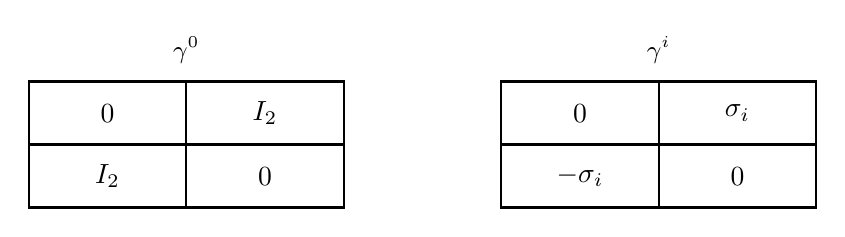
\begin{tikzpicture}[
    blk/.style={draw, thick, minimum width=1.8cm, minimum height=1.2cm, align=center},
    lab/.style={font=\small}
]
\node[lab] at (0,2.0) {\(\gamma^0\)};
\draw[thick] (-2,0) rectangle (2,1.6);
\draw[thick] (0,0) -- (0,1.6);
\draw[thick] (-2,0.8) -- (2,0.8);
\node at (-1,1.2) {\(0\)};
\node at (1,1.2) {\(\mathbb{I}_2\)};
\node at (-1,0.4) {\(\mathbb{I}_2\)};
\node at (1,0.4) {\(0\)};

\node[lab] at (6,2.0) {\(\gamma^i\)};
\draw[thick] (4,0) rectangle (8,1.6);
\draw[thick] (6,0) -- (6,1.6);
\draw[thick] (4,0.8) -- (8,0.8);
\node at (5,1.2) {\(0\)};
\node at (7,1.2) {\(\sigma_i\)};
\node at (5,0.4) {\(-\sigma_i\)};
\node at (7,0.4) {\(0\)};
\end{tikzpicture}
\caption{Forma en bloques de las matrices gamma en la base quiral.}
\end{figure}

\subsection{Chequeo del algebra de Clifford}
Ahora podemos verificar \eqref{c15:eq:cliff} de forma directa:
\begin{align}
(\gamma^0)^2 &= \beta^2 = \mathbb{I}_4,\\
\{\gamma^0,\gamma^i\}
&=
\beta(\beta\alpha^i)+(\beta\alpha^i)\beta
=
\alpha^i+\beta\alpha^i\beta
=
\alpha^i-\alpha^i
=0,\\
\{\gamma^i,\gamma^j\}
&=
\beta\alpha^i\beta\alpha^j+\beta\alpha^j\beta\alpha^i
=
-\alpha^i\alpha^j-\alpha^j\alpha^i
=
-2\delta^{ij}\mathbb{I}_4.
\end{align}

Ese signo menos en las componentes espaciales es exactamente el que distingue la metrica de Minkowski del caso euclideo. Esta es la primera señal fuerte de que ya entramos, al nivel efectivo, en el terreno relativista correcto.

\section{La ecuacion covariante}
\subsection{\texorpdfstring{Multiplicar por \(\beta\)}{Multiplicar por beta}}
Partimos de \eqref{c15:eq:hamiltonevo}:
\begin{equation}
i\partial_t \Psi =
\left(
-i\,v\,\alpha^i\partial_i + m\beta
\right)\Psi.
\end{equation}
Llevamos todo al mismo lado:
\begin{equation}
\left(
i\partial_t + i\,v\,\alpha^i\partial_i - m\beta
\right)\Psi=0.
\end{equation}
Multiplicamos por $\beta$ a la izquierda:
\begin{equation}
\left(
i\beta\partial_t + i\,v\,\beta\alpha^i\partial_i - m
\right)\Psi=0.
\end{equation}
Usando \eqref{c15:eq:defgamma}, esto queda
\begin{equation}
\left(
i\gamma^0\partial_t + i\,v\,\gamma^i\partial_i - m
\right)\Psi=0.
\label{c15:eq:almostcov}
\end{equation}

\subsection{Introducir una coordenada temporal efectiva}
Si definimos
\begin{equation}
x^0 = v t,
\qquad
\partial_0 = \frac{1}{v}\partial_t,
\end{equation}
la ecuacion \eqref{c15:eq:almostcov} toma la forma
\begin{equation}
\left(
i\gamma^0\partial_0 + i\gamma^i\partial_i - m
\right)\Psi=0.
\end{equation}
Reuniendo indice temporal y espaciales:
\begin{equation}
\boxed{
(i\gamma^\mu\partial_\mu - m)\Psi=0.
}
\label{c15:eq:diraccov}
\end{equation}

Ya llegamos exactamente a la ecuacion covariante de Dirac.

\begin{figure}[h!]
\centering
\begin{tikzpicture}[
    box/.style={draw, rounded corners, thick, align=center, minimum width=3.5cm, minimum height=1.2cm, fill=green!6},
    arr/.style={-{Latex[length=3mm]}, thick}
]
\node[box] (a) at (0,0) {\(i\partial_t\Psi=H\Psi\)};
\node[box] (b) at (4.6,0) {\(H=-iv\alpha^i\partial_i+m\beta\)};
\node[box] (c) at (9.2,0) {\(\gamma^0=\beta,\ \gamma^i=\beta\alpha^i\)};
\node[box] (d) at (13.8,0) {\((i\gamma^\mu\partial_\mu-m)\Psi=0\)};
\draw[arr] (a) -- (b);
\draw[arr] (b) -- (c);
\draw[arr] (c) -- (d);
\end{tikzpicture}
\caption{La traduccion algebraica del Hamiltoniano discreto-efectivo al lenguaje covariante.}
\end{figure}

\section{Quiralidad: donde viven los sectores de Weyl}
En la base quiral, la matriz
\begin{equation}
\gamma^5 = i\gamma^0\gamma^1\gamma^2\gamma^3
\end{equation}
toma la forma
\begin{equation}
\gamma^5=
\begin{pmatrix}
-\mathbb{I}_2 & 0\\
0 & \mathbb{I}_2
\end{pmatrix}.
\label{c15:eq:gamma5}
\end{equation}

Esto permite definir proyectores quirales:
\begin{equation}
P_L = \frac{1-\gamma^5}{2},
\qquad
P_R = \frac{1+\gamma^5}{2}.
\end{equation}
Aplicados al espinor completo, separan exactamente los dos sectores:
\begin{equation}
P_L\Psi=
\begin{pmatrix}
\psi_L\\
0
\end{pmatrix},
\qquad
P_R\Psi=
\begin{pmatrix}
0\\
\psi_R
\end{pmatrix}.
\end{equation}

En ausencia de masa, la ecuacion de Dirac se separa en dos ecuaciones de Weyl desacopladas. La masa es precisamente lo que mezcla ambos sectores. Esa es la razon profunda de que el termino masivo no sea un mero \enquote{ajuste energetico}, sino un acoplamiento estructural entre dos representaciones espinoriales distintas.

\begin{figure}[h!]
\centering
\begin{tikzpicture}[
    box/.style={draw, rounded corners, thick, align=center, minimum width=3.2cm, minimum height=1.4cm},
    arr/.style={-{Latex[length=3mm]}, thick}
]
\node[box, fill=blue!7] (L) at (0,0) {Sector izquierdo\\\(\psi_L\)\\\((1/2,0)\)};
\node[box, fill=red!7] (R) at (7,0) {Sector derecho\\\(\psi_R\)\\\((0,1/2)\)};
\draw[arr] (L) to[bend left=15] node[above] {\(m\)} (R);
\draw[arr] (R) to[bend left=15] node[below] {\(m\)} (L);
\node at (3.5,-2.1) {\(\Psi=\begin{pmatrix}\psi_L\\ \psi_R\end{pmatrix}\)};
\end{tikzpicture}
\caption{La masa acopla dos sectores quirales opuestos y produce un espinor de Dirac completo.}
\end{figure}

\section{\texorpdfstring{Donde entra realmente \(SL(2,\mathbb{C})\)}{Donde entra realmente SL(2,C)}}
\subsection{Primero: rotaciones}
En el limite efectivo, el termino $\bm{\sigma}\cdot\bm{q}$ ya nos dice que las matrices de Pauli implementan la forma espinorial de las rotaciones espaciales. La razon es que $SU(2)$ es el recubrimiento doble de $SO(3)$.

Eso es suficiente para entender por que un Hamiltoniano tipo Weyl transforma bien bajo rotaciones efectivas:
\begin{equation}
\psi \mapsto U\psi,
\qquad
U\in SU(2),
\end{equation}
mientras que $\bm{q}$ transforma como vector espacial.

\subsection{Despues: boosts y grupo de Lorentz}
Pero Dirac en \(3+1\) exige mas que rotaciones. Exige compatibilidad con todo el grupo de Lorentz $SO(3,1)$. Al nivel espinorial, el grupo que actua naturalmente no es $SO(3,1)$ sino su recubrimiento doble:
\begin{equation}
SL(2,\mathbb{C}) \longrightarrow SO^+(3,1).
\end{equation}

La condicion clave es que exista una accion espinorial $S(\Lambda)$ tal que
\begin{equation}
S(\Lambda)^{-1}\gamma^\mu S(\Lambda)=\Lambda^\mu{}_{\nu}\gamma^\nu.
\label{c15:eq:spinlorentz}
\end{equation}
Esta es la version compacta de \enquote{la ecuacion de Dirac tiene la simetria correcta}.

\subsection{La lectura de representaciones}
Los dos sectores Weyl que ya habiamos separado por quiralidad no transforman del mismo modo. Uno transforma en la representacion
\begin{equation}
\left(\frac{1}{2},0\right),
\end{equation}
y el otro en
\begin{equation}
\left(0,\frac{1}{2}\right).
\end{equation}

Una particula de Weyl usa solo uno de esos sectores. Una particula de Dirac usa ambos, empaquetados en un mismo espinor de cuatro componentes:
\begin{equation}
\Psi=
\begin{pmatrix}
\psi_L\\
\psi_R
\end{pmatrix}.
\end{equation}
Eso explica por que nuestro paso anterior, al duplicar la teoria y luego acoplarla, no era una maniobra artificial: era exactamente la operacion necesaria para pasar del lenguaje de Weyl al de Dirac.

\begin{figure}[h!]
\centering
\begin{tikzpicture}[
    box/.style={draw, rounded corners, thick, align=center, minimum width=3.3cm, minimum height=1.3cm},
    arr/.style={-{Latex[length=3mm]}, thick}
]
\node[box, fill=yellow!8] (lat) at (0,0) {Simetrias microscopicas\\de red};
\node[box, fill=green!8] (rot) at (4.5,0) {\(SO(3)\) efectivo\\y \(SU(2)\) espinorial};
\node[box, fill=blue!8] (lor) at (9,0) {\(SO(3,1)\) efectivo\\y \(SL(2,\mathbb{C})\)};
\node[box, fill=red!8] (dir) at (13.5,0) {Ecuacion de Dirac\\covariante};
\draw[arr] (lat) -- (rot);
\draw[arr] (rot) -- (lor);
\draw[arr] (lor) -- (dir);
\end{tikzpicture}
\caption{La jerarquia de grupos que no debemos perder de vista.}
\end{figure}

\section{Lo que este paso ya logro, y lo que aun no}
\subsection{Lo que ya quedo claro}
Con este capitulo ya fijamos de manera limpia el nucleo algebraico del objetivo:
\begin{enumerate}[label=\arabic*.]
    \item una dinamica discreta efectiva puede producir sectores tipo Weyl;
    \item dos sectores de quiralidad opuesta pueden reorganizarse como un espinor de Dirac;
    \item la masa acopla esos sectores;
    \item el Hamiltoniano en bloques se traduce exactamente a la ecuacion covariante \eqref{c15:eq:diraccov};
    \item la estructura relevante de grupos pasa de $SU(2)$ y rotaciones a $SL(2,\mathbb{C})$ y Lorentz.
\end{enumerate}

\subsection{Lo que todavia falta controlar}
Todavia no demostramos, en sentido fuerte, que una red microscopica concreta tenga toda esa simetria de Lorentz de forma emergente. Para eso quedan pendientes al menos cuatro cuestiones:
\begin{enumerate}[label=\arabic*.]
    \item isotropia efectiva suficientemente buena;
    \item control del doblamiento fermionico;
    \item identificacion precisa del limite continuo;
    \item derivacion de los generadores espinoriales de Lorentz a partir del modelo efectivo.
\end{enumerate}

En otras palabras: ya obtuvimos el blanco algebraico correcto, pero aun no cerramos todo el puente desde la microfisica discreta hasta la covariancia relativista completa.

\section{Mapa del siguiente paso}
El paso mas natural a partir de aqui es uno de estos:
\begin{enumerate}[label=\arabic*.]
    \item derivar explicitamente los generadores
    \(
    \Sigma^{\mu\nu}=\frac{i}{4}[\gamma^\mu,\gamma^\nu]
    \)
    y mostrar como codifican rotaciones y boosts;
    \item incorporar Nielsen--Ninomiya dentro de esta construccion concreta para ver como el doblamiento condiciona la aparicion de sectores Weyl;
    \item estudiar una realizacion discreta mas especifica donde la isotropia efectiva en \(3D\) quede mas controlada.
\end{enumerate}

\section{Resumen final}
El mensaje central de este capitulo es simple pero decisivo. El Hamiltoniano en bloques que obtuvimos al acoplar dos sectores Weyl no solo \enquote{se parece} al de Dirac: ya \emph{es} una realizacion concreta del algebra de Dirac. Al definir $\alpha^i$ y $\beta$, construir las matrices $\gamma^\mu$ y reagrupar la ecuacion de evolucion, aparece exactamente la forma covariante
\[
(i\gamma^\mu\partial_\mu-m)\Psi=0.
\]

Por eso este paso fija el centro algebraico del proyecto. La pregunta ya no es si el formalismo de Dirac puede aparecer; eso ya quedo mostrado. La pregunta ahora es cuan robustamente puede emerger desde una estructura discreta y que simetrias deben organizarse para que, en el limite adecuado, no solo aparezca un cono lineal, sino toda la arquitectura espinorial asociada a \(3+1\) dimensiones.
